\section{Ablation}
\label{sec:ablation}

The ablation removes one component of the protocol at a time and measures what is lost on the ten planted structures of
Section~\ref{sec:design-planted}. Table~\ref{tab:ablation} gives every variant and Figure~\ref{fig:coverage} the counts of the
first nine. The components are the sharp bounds, the second matrix, the $t$ rows, the single figures that the band replaces, the
common level and the tests.

\begin{table*}[htbp]
\centering
\small
\caption{What each component of the protocol contributes on the ten planted structures: for an interval, the number of structures whose capital it contains and its median width relative to the capital; for a single figure, the number within the stated tolerance and its median absolute relative error.}
\label{tab:ablation}
\fitwidth{\begin{tabular}{p{5.6cm}lcrp{3.4cm}}
\toprule
Variant & Covered when & Structures covered & Median width / error & Missed \\
\midrule
\relax full band (bounds and all interior rows, base and stressed matrix) & \relax contains the capital & \relax 10 of 10 & \relax 1.26 & \relax none \\
\relax without the sharp bounds (interior rows, base and stressed matrix) & \relax contains the capital & \relax 8 of 10 & \relax 0.17 & \relax Gaussian, independent risks; t copula, 3 degrees, crisis matrix \\
\relax without the stressed matrix (interior rows of the base matrix) & \relax contains the capital & \relax 2 of 10 & \relax 0.11 & \relax covers only Gaussian, base matrix; Gaussian regimes, 5 percent crisis \\
\relax without the t copula rows (square-root rule and Gaussian copula, base matrix) & \relax contains the capital & \relax 2 of 10 & \relax 0.07 & \relax covers only Gaussian, base matrix; Gaussian regimes, 5 percent crisis \\
\relax without the t copula rows, with the stressed matrix (square-root rule and Gaussian copula, both matrices) & \relax contains the capital & \relax 5 of 10 & \relax 0.14 & \relax covers only Gaussian, base matrix; Gaussian, market-credit 0.8; t copula, 3 degrees, base matrix; t copula, 2.5 degrees, base matrix; Gaussian regimes, 5 percent crisis \\
\relax t copula rows only (4, 8 and 30 degrees of freedom, both matrices) & \relax contains the capital & \relax 6 of 10 & \relax 0.15 & \relax covers only Gaussian, market-credit 0.8; Gaussian, crisis matrix; t copula, 3 degrees, base matrix; t copula, 2.5 degrees, base matrix; Clayton, reflected, same mean tau; Gumbel, same mean tau \\
\relax Gaussian copula row alone & \relax within 5 percent & \relax 2 of 10 & \relax 0.14 & \relax median error \\
\relax square-root row alone & \relax within 5 percent & \relax 2 of 10 & \relax 0.08 & \relax median error \\
\relax simple sum alone (the headline) & \relax within 5 percent & \relax 0 of 10 & \relax 0.18 & \relax median error \\
\relax hybrid quantile with the correlation of the truth sample & \relax within 5 percent & \relax 5 of 10 & \relax 0.07 & \relax median error \\
\relax Gaussian copula with the rank correlation of the truth sample & \relax within 5 percent & \relax 5 of 10 & \relax 0.04 & \relax median error \\
\relax Gaussian copula alone, tolerance 10 percent & \relax within 10 percent & \relax 2 of 10 & \relax 0.14 & \relax median error \\
\bottomrule
\end{tabular}}
\end{table*}


\begin{figure}[htbp]
\centering
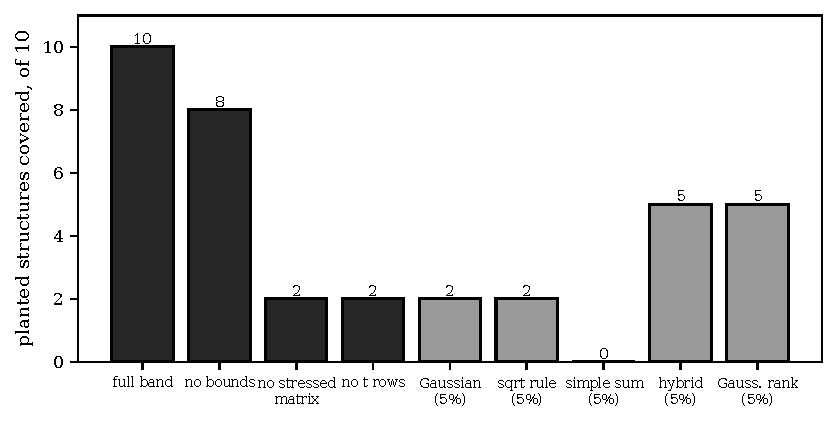
\includegraphics[width=0.9\textwidth]{figures/coverage}
\caption{Number of the ten planted structures covered by each variant: the full band and three intervals with one component removed (dark bars, containing the capital after widening by three standard errors), and five single figures (light bars, within 5 percent of the capital).}
\label{fig:coverage}
\end{figure}

\subsection{Components of the band read as an interval}
\label{sec:ablation-intervals}

The full band, with the bounds and the interior rows of both matrices, contains all ten capitals and has a median width of
$\bdAblFullWidth$ times the capital. Removing the sharp bounds leaves an interval of median width $\bdAblNoBoundsWidth$ that contains
$\bdAblNoBounds$ of the ten: it misses \bdMissedNoBounds{}, the structure with no dependence, which lies below every interior row, and
the heaviest tail, which lies above every interior row. The bounds therefore buy the last $\bdAblBoundsGain$ structures at a price of $\bdAblWidthBounds$ of the capital in median width, which is a high
price and a necessary one if coverage is the goal: no
choice of copula family and matrix can be known to span the structures that were not thought of, and the bounds are the only
rows that do not depend on that choice.

The stressed matrix is the component with the highest value for its width. Without it the interior rows of the base matrix
contain $\bdAblNoStress$ of the ten structures with a median width of $\bdAblNoStressWidth$; with it, and without the bounds, they
contain $\bdAblNoBounds$ at $\bdAblNoBoundsWidth$. The increase of $\bdAblStressGain$ structures costs $\bdAblWidthStress$ of the capital in median width. The $t$ rows have
the opposite profile on the base matrix: removing them leaves the square-root rule and the Gaussian row, which contain
$\bdAblNoT$ of the ten at a width of $\bdAblNoTWidth$, the same count as the five-row interval of the base matrix. Their
contribution appears in combination with the stressed matrix: without the $t$ rows but with both matrices the interval contains
$\bdAblNoTStress$ of the ten at a median width of $\bdAblNoTStressWidth$, against $\bdAblNoBounds$ for the five interior rows of
both matrices, and the $t$ rows alone, on both matrices, contain $\bdAblTOnly$ at $\bdAblTOnlyWidth$. The three components are
not additive, because each interior interval extends the others in different directions: the matrix moves the Gaussian
structures up, the $t$ rows move the capital of the heavy-tailed structures up, and neither can reach the independent case, which
only the bounds contain.

\subsection{Single figures against the band}
\label{sec:ablation-single}

A single figure is the alternative that the band replaces. Used alone and with a tolerance of 5 percent, the Gaussian copula row
is within the tolerance of $\bdAblGaussPoint$ of the ten structures, the square-root row of $\bdAblVcPoint$, the simple sum of
$\bdAblSumPoint$, the hybrid quantile calibrated on the structure of $\bdAblHybridPoint$ and the Gaussian copula calibrated on its rank
correlation of $\bdAblKendallPoint$. Loosening the tolerance of the Gaussian row to 10 percent does not change its count,
$\bdAblGaussTen$, because its errors are either below 2 percent or above 11 percent. The row that scores best as a point estimate when it
is calibrated on the structure, the Gaussian copula with the rank correlation of the structure, fails exactly on the structures
that Proposition~\ref{prop:tails} predicts it fails on, the five whose dependence has tail dependence, and the cost of that
failure is an underestimate of $\bdKTailMin$ to $\bdKTailMax$ percent. The interval is more informative than any of these figures because it states the
width of what is not known, and the width is the quantity that the single figures conceal: even the best calibrated estimator,
with a median error of $\bdKendallMedErr$ percent, has no indication of the 22 percent that it misses on the worst structure.
The comparison is conservative against the band, because the band's interior rows use named conventions while the competing
estimators use the structure's own data.

\subsection{The tests that each row feeds}
\label{sec:ablation-tests}

The tests of Section~\ref{sec:method-checks} each read a defined set of inputs, listed in Table~\ref{tab:tests-rows}. Removing the
$t$ rows leaves the copula-choice test unrunnable: the engine returns the light not evaluated when it is given an empty list of
$t$ capital figures. The correlation-stress test needs the Gaussian row of the stressed matrix, and the bracket test needs the two
bound rows, so removing the stressed band or the bounds leaves each without its input; these two are determined by the arguments
of the functions, which take the missing row as a required argument, and not by an engine call that refuses them. The first clause
of the prediction (H7) holds on these grounds.

\begin{table}[htbp]
\centering
\small
\caption{The nine tests of the aggregation battery, the rows or inputs each one reads, the light each returns on the committed aggregate and whether the test can be run when the Gaussian copula row is the only aggregate figure kept; the two amber lights belong to tests that read more than one row.}
\label{tab:tests-rows}
\fitwidth{\begin{tabular}{p{4.4cm}p{5.6cm}ll}
\toprule
Test of the aggregation battery & Inputs it reads & Light on the committed aggregate & Runs on the Gaussian row alone \\
\midrule
\relax simple sum and variance covariance & \relax Gaussian row; marginal capitals; correlation matrix & \relax green & \relax yes \\
\relax copula choice sensitivity & \relax Gaussian row; t rows & \relax amber & \relax no \\
\relax worst case bracket & \relax lower bound; worst case; interior rows & \relax green & \relax no \\
\relax correlation stress & \relax Gaussian row of the base matrix; Gaussian row of the stressed matrix & \relax amber & \relax no \\
\relax diversification sign & \relax the diversification factor of each interior row & \relax green & \relax yes \\
\relax horizon confidence consistency & \relax horizon and level of each marginal & \relax green & \relax yes \\
\relax euler additivity & \relax the Euler contributions and the aggregate expected shortfall & \relax green & \relax yes \\
\relax elliptical mc agreement & \relax square-root row; an elliptical simulation & \relax green & \relax yes \\
\relax rosenberg schuermann reference & \relax simple sum; Gaussian row & \relax green & \relax yes \\
\bottomrule
\end{tabular}}
\end{table}


The second clause was refuted. With the Gaussian row as the only aggregate figure kept, $\bdRunnableGaussOnly$ of the
$\bdTestsTotal$ tests still run, not at most half: the comparison with the simple sum and the square-root rule, the sign of the
diversification factors, the consistency of the horizon and the level, the additivity of the allocation, the agreement of a
Monte Carlo run with the square-root rule, and the reference of Rosenberg and Schuermann read the Gaussian row, the marginals or
the conventions. The prediction was mistaken about the proportion, not about the mechanism: the three tests that read the other
rows are the three that measure the dependence uncertainty (the sensitivity to the copula, the stress of the matrix and the bracket
of the bounds), and the six that run on a Gaussian row alone are those that verify arithmetic, units and a reference. The tests of the
dependence uncertainty are the ones that fail without the band.

\subsection{The common level and the allocation}
\label{sec:ablation-level}

The two remaining components were ablated in Section~\ref{sec:results}. Reading one marginal at another level changes the headline by
$\bdHeadlineChange$ percent and is caught twice, by the consistency test and by the refusal of the engine. The Euler allocation is
compared with the allocation by stand-alone expected shortfall, which sums to $\bdStandaloneOver$ times the aggregate and so is not
an allocation of it; the Euler allocation adds up to the aggregate in every seed to a relative $\bdEulerMaxGap$, and its price is
a sampling standard deviation of $\bdShareSdMin$ to $\bdShareSdMax$ percentage points in a share, because it rests on the same thousand tail draws as the
value at risk. Neither ablation changes a row of the band: the level check protects the inputs and the allocation extends the
output. Their value is that they close two routes by which a correct band can be misread, a headline built from marginals at
different levels, which no row would reveal because every row inherits it, and an allocation whose parts do not sum to the whole,
which a reader would otherwise normalise by eye. The refusal of the engine for an unconverted capital is the stronger of the two
defences on the level, since it holds when the metadata of the marginals are wrong.
